\section{آموزش شبکه عصبی}
\label{sec:training}

در این بخش، پس از تعریف معماری شبکه، به آموزش آن پرداخته می‌شود. ابتدا تنظیمات و پارامترهای آموزش معرفی می‌شوند و سپس روند آموزش، نقش داده‌های اعتبارسنجی، نحوه تعیین بسامد اعتبارسنجی و توابع مورد استفاده برای محاسبه و پایش خطا توضیح داده می‌شود.

\subsection{تنظیمات آموزش}

پس از تعیین معماری شبکه، لازم است تنظیمات مربوط به فرایند یادگیری مشخص شوند. پارامترهای مورد استفاده برای تنظیم فرایند آموزش در این مثال عبارت‌اند از:

\begin{enumerate}
\item \textbf{الگوریتم بهینه‌سازی}: این الگوریتم نحوه به‌روزرسانی وزن‌های شبکه را در فرایند یادگیری تعیین می‌کند. در این مثال از الگوریتم \lr{Adam} استفاده شده است که وزن‌های شبکه را در طول آموزش به‌روزرسانی می‌کند تا مقدار خطا کاهش یابد.
\item \lr{\textbf{MaxEpochs}}: تعداد دفعات عبور از کل مجموعه آموزشی را مشخص می‌کند. در این مثال، حداکثر تعداد تکرارها برابر با ۱۰۰ است؛ بااین‌حال، در صورت فعال‌شدن شرط توقف زودهنگام، آموزش ممکن است پیش از رسیدن به این تعداد متوقف شود.
\item \lr{\textbf{MiniBatchSize}}: تمام داده‌ها به‌صورت یک‌جا وارد شبکه عصبی نمی‌شوند؛ بلکه به دسته‌هایی تقسیم می‌شوند و هر دسته به‌طور جداگانه به شبکه داده می‌شود. در این مثال، اندازه هر دسته برابر با ۲۵۶ نمونه است.
\item \lr{\textbf{Metrics}}: معیار \lr{RMSE} برای پایش عملکرد مدل در طول آموزش مورد استفاده قرار می‌گیرد.
\item \lr{\textbf{Shuffle}}: پس از هر \lr{epoch}، ترتیب داده‌ها را تغییر می‌دهد تا فرایند آموزش به ترتیب ثابتی از نمونه‌ها وابسته نباشد.
\item \lr{\textbf{InitialLearnRate}}: این پارامتر نرخ تغییر وزن‌های شبکه را در فرایند بهینه‌سازی کنترل می‌کند.
\item \lr{\textbf{OutputNetwork}}: بهترین عملکرد شبکه لزوماً در آخرین \lr{epoch} (یعنی \lr{epoch = 100}) حاصل نمی‌شود. این پارامتر شبکه‌ای را که بر اساس معیار اعتبارسنجی بهترین عملکرد را داشته است، به‌عنوان خروجی انتخاب می‌کند.
\item \lr{\textbf{ValidationData}}: مجموعه داده اعتبارسنجی را مشخص می‌کند. این داده‌ها برای ارزیابی عملکرد مدل به کار می‌روند و در به‌روزرسانی وزن‌های شبکه نقشی ندارند.
\item \lr{\textbf{ValidationFrequency}}: مشخص می‌کند فرایند اعتبارسنجی پس از چند مرحله آموزش انجام شود.
\item \lr{\textbf{ValidationPatience}}: این پارامتر برای اعمال توقف زودهنگام به کار می‌رود. مقدار ۱۰ به این معناست که اگر معیار اعتبارسنجی طی ۱۰ نوبت متوالی بهبود نیابد، آموزش متوقف می‌شود.
\end{enumerate}

در نهایت، ورودی‌ها، پارامترها، مقادیر مورد انتظار و معماری شبکه، به همراه تابع زیان \lr{MAE}، برای اجرای فرایند آموزش به کار گرفته می‌شوند.

\subsection{روند آموزش}

پس از آغاز آموزش مدل، روند یادگیری را می‌توان در دو نمودار مربوط به \lr{RMSE} و \lr{loss} مشاهده کرد. تابع زیان مورد استفاده در این آموزش از نوع \lr{MAE} است. در هر دو نمودار، مقادیر مربوط به مجموعه آموزش (\lr{Training}) و مجموعه اعتبارسنجی (\lr{Validation}) نمایش داده شده‌اند. شکل~\ref{fig:training} تغییرات این دو معیار را در طول تکرارهای آموزش نشان می‌دهد؛ نمودار بالایی مربوط به \lr{RMSE} و نمودار پایینی مربوط به تابع زیان است.

\begin{figure}[!htbp]
\centering
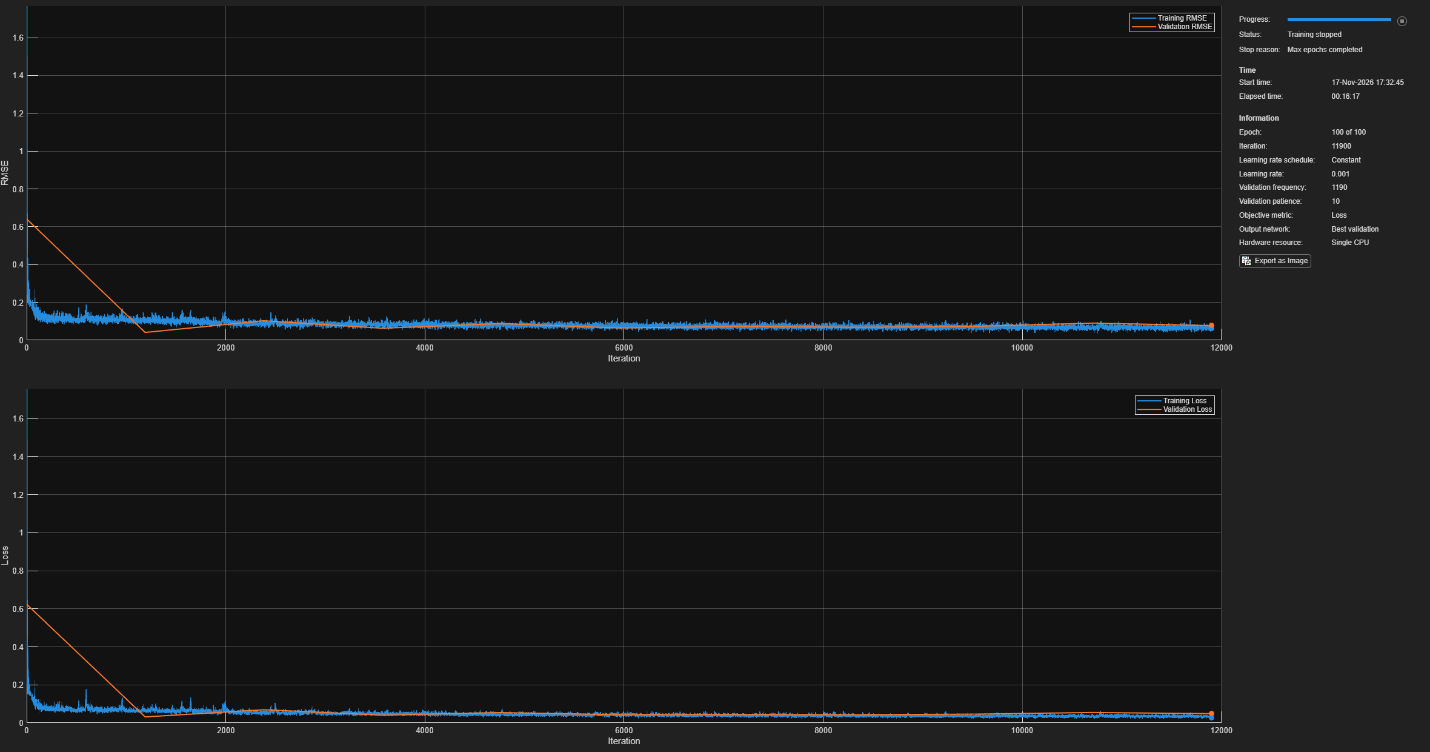
\includegraphics[width=\textwidth]{img/training.png}
\caption{روند تغییرات معیار RMSE (و تابع زیان (نمودار پایین) برای مجموعه‌های آموزش و اعتبارسنجی.}
\label{fig:training}
\end{figure}

\subsection{نقش داده‌های اعتبارسنجی}

با توجه به اینکه داده‌های اعتبارسنجی در به‌روزرسانی وزن‌های مدل نقشی ندارند، استفاده از آن‌ها در فرایند آموزش چه ضرورتی دارد؟

نمونه‌های اعتبارسنجی با استفاده از شاخص‌های از پیش تعیین‌شده انتخاب شده‌اند و با داده‌های آموزش هم‌پوشانی ندارند. اهمیت این موضوع در آن است که ممکن است خطای آموزش کاهش یابد و نشان دهد مدل روی داده‌های آموزشی عملکرد مناسبی دارد؛ اما اگر خطای اعتبارسنجی کاهش نیابد یا افزایش پیدا کند، می‌توان احتمال داد که مدل به‌جای یادگیری الگوهای قابل تعمیم، بیش از حد با داده‌های آموزشی سازگار شده است؛ به‌عبارت دیگر، دچار بیش‌برازش\LTRfootnote{Overfitting} شده است.

بنابراین، اعتبارسنجی نوعی بازخورد درباره عملکرد شبکه فراهم می‌کند، اما مستقیماً وزن‌های آن را تغییر نمی‌دهد.

\subsection{تعیین مقدار \lr{ValidationFrequency}}

همان‌طور که در بخش تنظیمات آموزش اشاره شد، پارامتر \lr{ValidationFrequency} مشخص می‌کند ارزیابی پس از چند مرحله آموزش انجام شود. در این مثال، مقدار این پارامتر با استفاده از دستور زیر محاسبه می‌شود:

\begin{center}
\lr{\small\texttt{validationFrequency = 10*floor(numel(trainRulData)/miniBatchSize);}}
\end{center}

تعداد نمونه‌های موجود در \lr{trainRulData} تقریباً برابر با ۳۰٬۰۰۰ است (مقدار دقیق آن ۳۰٬۷۰۶ نمونه است). این تعداد از مجموع چرخه‌های مربوط به ۳۰ باتری مجموعه آموزش به دست می‌آید؛ به‌طور متوسط، برای هر باتری حدود ۱۰۰۰ چرخه در نظر گرفته شده است. اطلاعات هر چرخه نیز در مراحل پیشین به‌صورت یک ماتریس آماده شده‌اند. بنابراین، ابعاد داده‌های ورودی شبکه عصبی برابر با $30\times30\times3\times30706$ خواهد بود.

اندازه هر دسته (\lr{batch}) برابر با ۲۵۶ نمونه در نظر گرفته شده است:
\[
\frac{30706}{256} = 119.945
\]
\[
\lfloor 119.945 \rfloor = 119
\]
\[
\mathrm{validationFrequency} = 10 \times 119 = 1190
\]

این مقدار به آن معناست که پس از هر ۱۱۹۰ دسته آموزشی، یک‌بار ارزیابی با استفاده از داده‌های اعتبارسنجی انجام می‌شود؛ به‌عبارت دیگر، اعتبارسنجی تقریباً هر ۱۰ \lr{epoch} یک‌بار تکرار خواهد شد و در طول ۱۰۰ \lr{epoch}، حدود ۱۰ بار انجام می‌شود. با توجه به اینکه مقدار \lr{ValidationPatience} برابر با ۱۰ است، سازوکار توقف زودهنگام در بازه ۱۰۰ \lr{epoch} فرصت محدودی برای فعال‌شدن خواهد داشت. بنابراین، انتظار می‌رود آموزش در بسیاری از اجراها تا سقف ۱۰۰ \lr{epoch} ادامه یابد.

\subsection{تابع زیان و معیار پایش}

برای آموزش این مدل از تابع \lr{MAE} استفاده شده است. این معیار میانگین قدرمطلق اختلاف میان مقادیر واقعی و پیش‌بینی‌شده را مطابق رابطه~\eqref{eq:mae} محاسبه می‌کند:
\begin{equation}
\mathrm{MAE} = \frac{1}{n}\sum_{i=1}^{n}\left| y_i - \hat{y}_i \right|
\label{eq:mae}
\end{equation}
الگوریتم \lr{Adam} با به‌روزرسانی وزن‌های شبکه، مقدار این تابع زیان را کاهش می‌دهد. علاوه بر این، برای پایش عملکرد مدل از معیار \lr{RMSE} نیز استفاده می‌شود. مطابق رابطه~\eqref{eq:rmse}، در این معیار ابتدا میانگین مربع خطاها محاسبه و سپس از آن جذر گرفته می‌شود:
\begin{equation}
\mathrm{RMSE} = \sqrt{\frac{1}{n}\sum_{i=1}^{n}\left( y_i - \hat{y}_i \right)^{2}}
\label{eq:rmse}
\end{equation}
در این روابط، $y_i$ مقدار واقعی و $\hat{y}_i$ مقدار پیش‌بینی‌شده برای نمونه $i$ است. ازاین‌رو، \lr{RMSE} نسبت به خطاهای بزرگ حساسیت بیشتری دارد. اگر مقدار این معیار به \lr{MAE} نزدیک باشد، معمولاً نشان می‌دهد اندازه خطاها چندان پراکنده نیست؛ اما اگر \lr{RMSE} به‌طور محسوسی بزرگ‌تر از \lr{MAE} باشد، احتمال وجود چند خطای بزرگ در میان پیش‌بینی‌ها مطرح می‌شود. بنابراین، بررسی \lr{RMSE} در کنار \lr{MAE} اطلاعات کامل‌تری درباره توزیع خطاها فراهم می‌کند.
